\normaltrue \difficilefalse \tdifficilefalse
\correctionfalse
%\UPSTIidClasse{11} % 11 sup, 12 spé
%\newcommand{\UPSTIidClasse}{11}

\exer{ $\star$ \label{B2:16:72}}
%% CCP MP 2007
\setcounter{numques}{0}
\UPSTIcompetence[2]{B2-16}
\index{Compétence B2-16}

\index{Tripteor}
\index{Hyperstatisme}

\ifcorrection
\else
\textbf{Pas de corrigé pour cet exercice.}
\fi

Le triptéor est un centre d'Usinage Grande Vitesse à architecture parallèle, permettent d'envisager un usinage rapide et précis.


\begin{figure}[H]
\centering
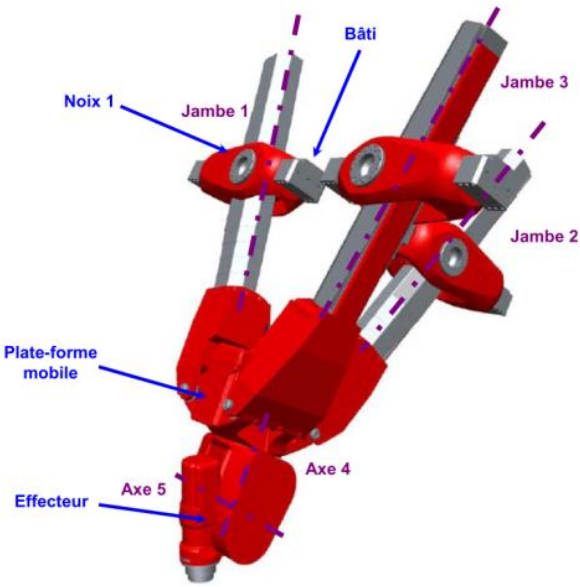
\includegraphics[width=\linewidth]{72_01.png}
%\caption{Pince utilisée sur le système ROBOVOLC et schéma cinématique associé \label{fig_23}}
\end{figure} 

\begin{figure}[H]
\centering
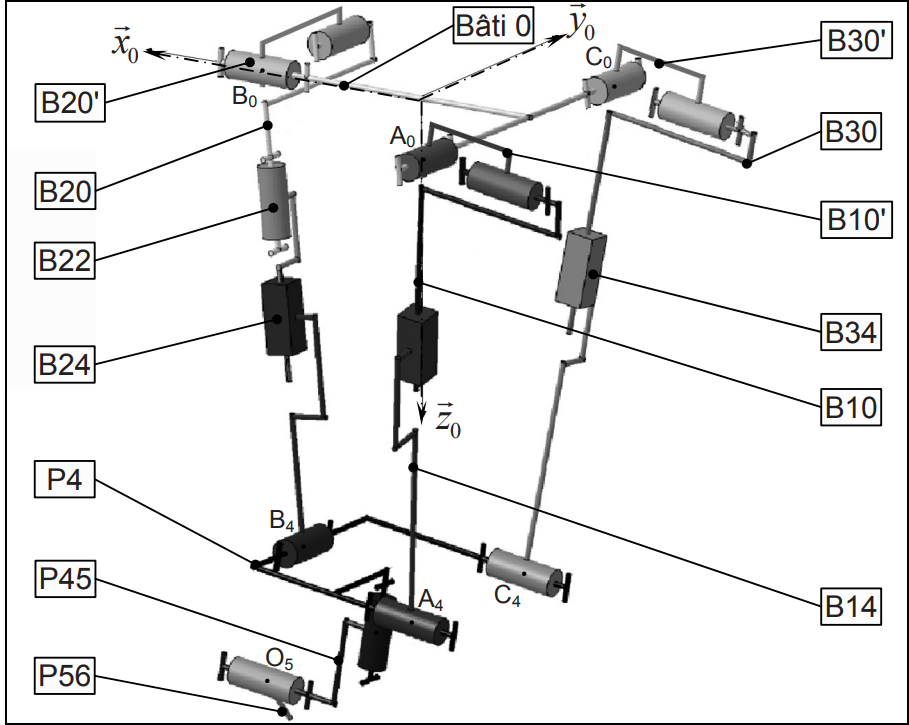
\includegraphics[width=\linewidth]{72_02.png}
%\caption{Pince utilisée sur le système ROBOVOLC et schéma cinématique associé \label{fig_23}}
\end{figure} 

\question{Réaliser le graphe de liaisons.}

\question{Calculer le degré d'hyperstatisme.}

 

\ifprof
\else

\noindent\footnotesize
 \fbox{\parbox{.9\linewidth}{
 Éléments de corrigé : 
 \begin{enumerate}
\item .
%\item $h=8$.
\item .
 \end{enumerate}}}
\normalsize

\begin{flushright}
\footnotesize{Corrigé  voir \ref{B2:16:72}.}
\end{flushright}%
\fi